
%(BEGIN_QUESTION)
% Copyright 2007, Tony R. Kuphaldt, released under the Creative Commons Attribution License (v 1.0)
% This means you may do almost anything with this work of mine, so long as you give me proper credit

Suppose this current-to-pressure (I/P) transducer's force coil suddenly fails open:

$$\includegraphics[width=15.5cm]{i01618x01.eps}$$

\noindent
Choose the best answer to describe the effects of this fault:

\begin{itemize}
\item{} The output pressure will fall all the way to zero PSI
\vskip 10pt
\item{} The output pressure will increase slightly 
\vskip 10pt
\item{} The output pressure will rise all the way to full supply PSI 
\vskip 10pt
\item{} The output pressure will decrease slightly 
\vskip 10pt
\item{} There will be no effect whatsoever -- all will continue as normal
\end{itemize}


\underbar{file i01618}
%(END_QUESTION)





%(BEGIN_ANSWER)

The output pressure will fall all the way to zero PSI

%(END_ANSWER)





%(BEGIN_NOTES)

{\bf This question is intended for exams only and not worksheets!}.

%(END_NOTES)


